\documentclass[border=7pt]{standalone}
\usepackage{amsmath,amssymb,bm,mathtools}
\usepackage[fontset=none]{ctex}
\setCJKmainfont{Songti SC}\setCJKsansfont{PingFang SC}
\usepackage{tikz}\usetikzlibrary{arrows.meta,calc,patterns,angles,quotes,decorations.markings,decorations.pathmorphing}
\newcommand{\dd}{\mathop{}\!\mathrm d}
\definecolor{blue}{HTML}{235789}\definecolor{red}{HTML}{BC4B41}
\tikzset{axis/.style={->,>=Stealth,line width=.55pt},world/.style={line width=.9pt},flow/.style={->,>=Stealth,line width=.85pt},ray/.style={->,>=Stealth,line width=.85pt},guide/.style={dashed,line width=.4pt},aux/.style={dashed,line width=.4pt},dim/.style={<->,>=Stealth,line width=.5pt},every node/.style={font=\normalsize},force/.style={->,>=Stealth,very thick},gas/.style={fill=blue!7}}
\begin{document}
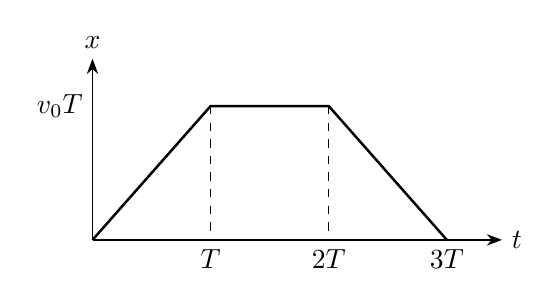
\begin{tikzpicture}\draw[axis](0,0)--(5.2,0)node[right]{$t$};\draw[axis](0,0)--(0,2.3)node[above]{$x$};\draw[world](0,0)--(1.5,1.7)--(3,1.7)--(4.5,0);\draw[guide](1.5,1.7)--(1.5,0) (3,1.7)--(3,0);\node[left]at(0,1.7){$v_0T$};\node[below]at(1.5,0){$T$};\node[below]at(3,0){$2T$};\node[below]at(4.5,0){$3T$};\end{tikzpicture}
\end{document}
